\documentclass[xcolor=svgnames,dvipsnames,table, hyperref=pdftex, mathserif, presentation]{beamer}
\usepackage{amsmath,amssymb,amsfonts,amsthm}
\usepackage{ctex}
\setCJKsansfont{KaiTi}% 文泉驿的黑体
\usepackage{graphics}
\usepackage{graphicx}
\usepackage{xcolor}
\usepackage{wasysym}
\usepackage{bbm}
\usepackage{url}
\usepackage{beamerleanprogress}
\usepackage{tikz-dependency}
\usepackage{tikz-qtree}
\usepackage{hhline}
\usepackage{fancyvrb}
\usepackage{mathrsfs}
\usepackage{alltt}

\usetheme{CambridgeUS}
%\usetheme{Pittsburgh}
\usecolortheme{orchid} % seahorse  orchid rose
\setbeamertemplate{blocks}[rounded][shadow=true]
\AtBeginSection[]{%
  \begin{frame}<beamer>
    \frametitle{Outline}
      \tableofcontents[current] 
    \end{frame}
  \addtocounter{framenumber}{-1}% If you don't want them to affect the slide number
}
\AtBeginSubsection[]
{
  \begin{frame}
  \frametitle{Outline}
    \tableofcontents[currentsection,currentsubsection]
  %\tableofcontents[sectionstyle=show/hide,subsectionstyle=hide/show/hide]
  \end{frame}
  \addtocounter{framenumber}{-1}% If you don't want them to affect the slide number
}
\newcommand{\setof}[1]{\ensuremath{\left \{ #1 \right \}}}
\newcommand{\tuple}[1]{\ensuremath{\left \langle #1 \right \rangle }}
\newcommand{\red}[1]{\textcolor{red}{#1}}
\newcommand{\brown}[1]{\textcolor{brown}{#1}}
\newcommand{\green}[1]{\textcolor{green}{#1}}
\newcommand{\blue}[1]{\textcolor{blue}{#1}}
\newcommand{\cyan}[1]{\textcolor{cyan}{#1}}

%gets rid of navigation symbols
%\setbeamertemplate{navigation symbols}{}

\begin{document}

\title[MF+FOL]{Injecting Logical Background for Relation Extraction}

\institute[icst.wip@pku]{
  
}
\author[Tim Rockt]{
  Tim Rockt aschel (UCL)\\
  Sameer Singh (UW)\\
  Sebastian Riedel (UCL)\\ 
}

\frame[t,plain]{ \titlepage } % [t,plain]

\frame{
  \frametitle{ Outline  }
  
   \begin{itemize}
      \item 论文概述
      \item 矩阵分解(Matrix factorization), 一阶谓词逻辑(first-order logic)
      \item 符号集(Notation)
      \item 一阶谓词逻辑注入(Inject)矩阵分解
	  \begin{itemize}
	   \item 矩阵分解之前操作(Pre-Factorization)
	   \item 融入矩阵分解之中('joint')
	  \end{itemize}

      \item 实验
	  \begin{itemize}
	   \item 预处理,规则生成,评价
	  \end{itemize}
   \end{itemize}

}

\frame{
  \frametitle{ summary }
  \centering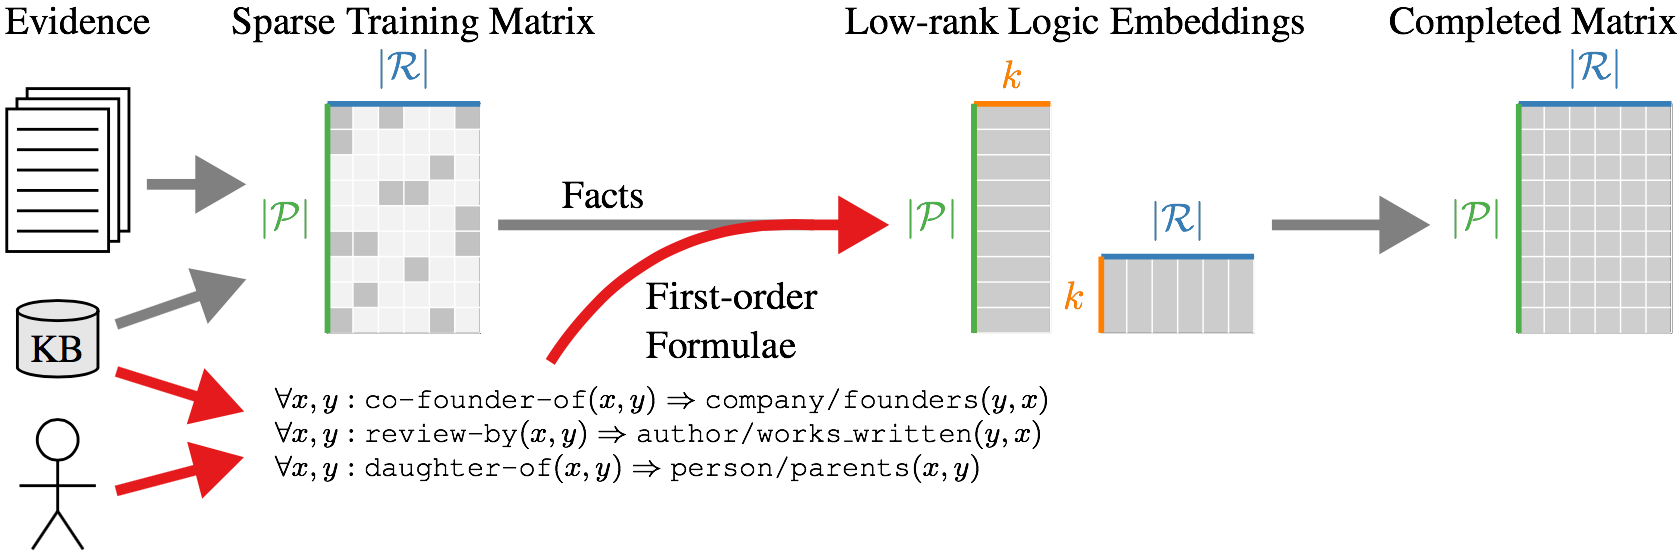
\includegraphics[width=0.9\hsize]{file/overview.png}
  
  
  原始矩阵 $|\mathcal{P}|\times|\mathcal{R}|$ \\
\resizebox{6cm}{!}{
\begin{tabular}{l|l|l|r|l|l|l|l|l|l|}
\multicolumn{1}{c}{} & \multicolumn{1}{c}{fr1}  & \multicolumn{1}{c}{fr2}  & \multicolumn{1}{c}{fr3}  & \multicolumn{1}{c}{p1}  & \multicolumn{1}{c}{p2}  & \multicolumn{1}{c}{p3}  & \multicolumn{1}{c}{p4}  & \multicolumn{1}{c}{p5}  & \multicolumn{1}{c}{p6} \tabularnewline \hhline{~|*{9}{-}}
\rowcolor[HTML]{C0C0C0} 
(e1,e2)  & \cellcolor[HTML]{EFEFEF}1 & \cellcolor[HTML]{EFEFEF}0 & \cellcolor[HTML]{EFEFEF}0                      & 0  & 1  & 0  & 0  & 1  & 0  \tabularnewline \hhline{~|*{9}{-}}
\rowcolor[HTML]{C0C0C0} 
(e2,e3)  & \cellcolor[HTML]{EFEFEF}0 & \cellcolor[HTML]{EFEFEF}1 & \cellcolor[HTML]{EFEFEF}0                      & 1  & 0  & 0  & 1  & 0  & 0  \tabularnewline \hhline{~|*{9}{-}}
\rowcolor[HTML]{C0C0C0} 
(e1,e3)  & \cellcolor[HTML]{EFEFEF}0 & \cellcolor[HTML]{EFEFEF}0 & \cellcolor[HTML]{EFEFEF}1                      & 0  & 0  & 1  & 0  & 0  & 0  \tabularnewline \hhline{~|*{9}{-}}
\rowcolor[HTML]{C0C0C0} 
(e1,e10) & \cellcolor[HTML]{EFEFEF}1 & \cellcolor[HTML]{EFEFEF}0 & \cellcolor[HTML]{EFEFEF}0                      & 1  & 0  & 0  & 0  & 0  & 0  \tabularnewline \hhline{~|*{9}{-}}
(e1,e6)  & \cellcolor[HTML]{FFCCC9}1 & \cellcolor[HTML]{FFCCC9}1 & \cellcolor[HTML]{FFCCC9}0                      & 1  & 0  & 0  & 1  & 1  & 0  \tabularnewline \hhline{~|*{9}{-}}
(e1,e8)  & \cellcolor[HTML]{FFCCC9}1 & \cellcolor[HTML]{FFCCC9}0 & \cellcolor[HTML]{FFCCC9}0                      & 1  & 0  & 0  & 0  & 0  & 0  \tabularnewline \hhline{~|*{9}{-}} 
(e3,e7)  & \cellcolor[HTML]{FFCCC9}0 & \cellcolor[HTML]{FFCCC9}1 & \cellcolor[HTML]{FFCCC9}0 & 1  & 0  & 0  & 1  & 0  & 0  \tabularnewline \hhline{~|*{9}{-}}
\end{tabular}
}

}

\frame{
  \begin{itemize}
   \item 矩阵分解(MF) vs 规则抽取(Rule-based)
      \begin{itemize}
       \item MF: 开放域、不需要标注数据(弱监督);完全依赖于KB的质量
	  \begin{itemize}
	   \item 关系出现次数多,预测才好;不出现的无法预测;
	  \end{itemize}

       \item Rule-based: 可以发现新的实体,新的关系;噪声大
      \end{itemize}
   \item 本文动机
      \begin{itemize}
       \item 矩阵分解 和 规则(一阶逻辑) 混合
      \end{itemize}
   \item 本文的贡献
      \begin{enumerate}
       \item 如何在矩阵分解前、后利用谓词逻辑
       \item 利用一阶谓词逻辑训练更好的实体对向量、谓词向量
       \item 结合MF,FOL来预测实体的关系
      \end{enumerate}

  \end{itemize}

}

\frame{
  \frametitle{ Notation}
  $\mathcal{P}\subseteq\varepsilon\times\varepsilon$ :实体对$(e_i,e_j)$集合 \\
  $\mathcal{R}$ :关系$fr_i,p_j$集合 \\
  $V$:向量空间$\{v_{fr_1}=\mathbf{v_{r_m}},v_{fr_2},...,v_{p_1}=\mathbf{v_{(e_i,e_j)}},v_{p_2},...\}$ \\
  $\pi_{m}^{e_i,e_j}=\sigma(\mathbf{v_{r_m}},\mathbf{v_{(e_i,e_j)}})$ :实体对与关系的相似性 $\sigma$:sigmoid func
  \begin{itemize}
   \item 一阶谓词
      \begin{itemize}
	\item 原子问题(ground Atom):$professorAt(x,y)$
	\item 复合问题(logical background knowledge):$professorAt(x,y)\Rightarrow emplyeeAt(x,y)$
      \end{itemize}
  \end{itemize}
   评价一阶谓词子集$\mathbf{w}$的好坏 $$p(\mathbf{w}|{V})=\prod_{r_m(e_i,e_j)\in w}\pi_{m}^{e_i,e_j}\prod_{r_m(e_i,e_j)\notin w}(1-\pi_{m}^{e_i,e_j})$$
  
}

\frame{
  \frametitle{ Method }
  \begin{enumerate}
   \item 传统方法
      \begin{itemize}
       \item 直接矩阵分解(MF)
       \item 只利用逻辑规则(Inf)
      \end{itemize}
   \item FOL,MF “混合”模型
      \begin{enumerate}
	\item FOL作为预处理 (Pre-Factorization Inference)
	  \begin{itemize}
	  \item 先用FOL改变原始矩阵 $M_{|\mathcal{P}|\times|\mathcal{R}|}$ ,再进行普通矩阵分解
	  \end{itemize}
       \item 一阶谓词子集加入目标函数(Joint Optimization)
       \item 传统矩阵分解生成向量空间$V$,然后使用收集的逻辑规则预测(Post-Factorization Inference)
      \end{enumerate}

  \end{enumerate}

}

\frame{
  \frametitle{一阶逻辑(FOL)注入}
  两种途径\\
      \begin{enumerate}
	\item FOL作为预处理 (Pre-Factorization Inference)
	  \begin{itemize}
	  \item 先用FOL改变原始矩阵 $M_{|\mathcal{P}|\times|\mathcal{R}|}$ ,再进行普通矩阵分解
	  \end{itemize}
       \item 一阶谓词子集加入目标函数(Joint Optimization)
      \end{enumerate}
  
}

\frame{
  \frametitle{Pre-Factorization Inference(FOL作为预处理)}
  核心:弥补矩阵的稀疏性,增加收集的\emph{一阶逻辑规则}与freebase relation之间的关联 \\
  方法:根据逻辑规则,增加原始矩阵 $M_{|\mathcal{P}|\times|\mathcal{R}|}$中值为1的元素个数
  \begin{block}{步骤}
   \begin{itemize}
    \item 收集一阶谓词规则
    \item 对每一条规则,比如$\mathbf{F}=\forall x,y:r_s(x,y) \Rightarrow (x,y)$
	\begin{itemize}
	 \item 如果$[(x,y),r_s]$上的值为1,则把$[(x,y),r_t]$上的值置为1
	 \item 递归做下去,知道没有新的1出现
	\end{itemize}
    \item 对更新后的矩阵$M_{|\mathcal{P}|\times|\mathcal{R}|}'$进行矩阵分解
   \end{itemize}

  \end{block}

}

\frame{
  \frametitle{Joint Optimization(组合模型)}
  核心:把收集的\emph{一阶逻辑规则}加入到矩阵分解的目标函数中\\
  训练集的目标函数:$$\displaystyle\min_V \sum_{\mathcal{F}\in\mathfrak{F}}\mathcal{L}([\mathcal{F}])$$
  \begin{block}{}
  \small $[\mathcal{F}]$ is the marginal probability $p(w|V)$ that the formula F is true under the model
  \end{block}
  $\mathcal{L}([\mathcal{F}]:=-\log([\mathcal{F}])$\\
  $p(\mathbf{w}|{V})=\prod_{r_m(e_i,e_j)\in w}\pi_{m}^{e_i,e_j}\prod_{r_m(e_i,e_j)\notin w}(1-\pi_{m}^{e_i,e_j})$
  
}

\frame{
  \frametitle{边缘分布(marginal probability)}
  \begin{block}{definition}
   对多变量的分布函数,针对某个变量进行求和\emph{(枚举其他变量的所有情况)},所得到的概率分布
  \end{block}
  
  \begin{block}{example}
   联合概率$P(A,B)$,对A的边缘分布为$P_1(A)=\sum_{b\in B}P(A,b)$,对B的边缘分布为$P_2(B)=\sum_{a\in A}P(a,B)$
  \end{block}
  

}

\frame{
  \frametitle{边缘分布(marginal probability)}
  \begin{block}{}
   $p(\mathbf{w}|{V})=\prod_{r_m(e_i,e_j)\in w}\pi_{m}^{e_i,e_j}\prod_{r_m(e_i,e_j)\notin w}(1-\pi_{m}^{e_i,e_j})$\\
  $p(\mathbf{w}|{V})=\prod f_{r_m(e_i,e_j)}=f_{r_m(e_i,e_j)}\times f_{r_n(e_k,e_l)}\times ...$\\
   \begin{tiny}
   \begin{equation}
    f_{r_m(e_i,e_j)}=
   \begin{cases}
   \pi_{m}^{e_i,e_j} &\mbox{if $r_m(e_i,e_j)\in w$ }\\
   1-\pi_{m}^{e_i,e_j} &\mbox{if $r_m(e_i,e_j)\notin w$ }\\
   \end{cases}
  \end{equation}
  \end{tiny}
  \end{block}
 
 \begin{itemize}
  \item 当$\mathcal{F}$是原子命题时 $[\mathcal{F}]=\pi_{m}^{e_i,e_j}$\\
  \item 当$\mathcal{F}=\mathcal{A}\wedge\mathcal{B}$, $\mathcal{A}$和$\mathcal{B}$是原子命题时, $[\mathcal{F}]=\pi_{m}^{e_i,e_j}\times\pi_{m}^{e_i,e_j}=[\mathcal{A}][\mathcal{B}]$\\
  \item 当$\mathcal{F}=\neg\mathcal{A}$,$\mathcal{A}$是原子命题时,$[\mathcal{F}]=1-[\mathcal{A}]$
  \item $\mathcal{F}=\mathcal{A}\vee\mathcal{B}=1-(\neg\mathcal{A})\wedge(\neg\mathcal{B})$
 \end{itemize}

  \begin{block}{}
  $[\mathcal{A}\vee\mathcal{B}]=[\mathcal{A}]+[\mathcal{B}]-[\mathcal{A}][\mathcal{B}]$\\
  $[\mathcal{A}\Rightarrow\mathcal{B}]=[\mathcal{A}]([\mathcal{B}]-1)+1$\\
  ...
  \end{block}

  
  

  
}
\frame{
  \frametitle{Joint Optimization(组合模型)}
  目标函数:$$\displaystyle\min_V \sum_{\mathcal{F}\in\mathfrak{F}}\mathcal{L}([\mathcal{F}])$$
  使用随机梯度下降(stochastic gradient descent)求解
  \begin{block}{}
   \begin{itemize}
    \item 对任意一个$\mathcal{F}$,其只和实体对向量、谓词向量有关
    \item 对任意$\mathcal{L}([\mathcal{F}])$只要求$\partial \mathcal{L}([\mathcal{F}])/\partial v_{r_m}$和$\partial\mathcal{L}([\mathcal{F}])/\partial v_{(e_i,e_j)}$
   \end{itemize}

  \end{block}

}




\frame{
  \frametitle{ }
  
\begin{tabular}{c|c|c|c|cc|}
    \multicolumn{1}{c}{} & \multicolumn{1}{c}{A} & \multicolumn{1}{c}{B} & \multicolumn{1}{c}{C} &           D           & \multicolumn{1}{c}{E} \tabularnewline \hhline{~|*{5}{-}}
             a           &  \cellcolor{blue!25}  & \multicolumn{1}{c}{}  & \multicolumn{1}{c}{}  &                       &  \cellcolor{red!25}   \tabularnewline \cline{2-3}
             b           &   \cellcolor{green!25}                    &            \cellcolor{green!25}           & \multicolumn{1}{c}{}  &                       &  \tabularnewline \cline{2-4}
             c           &  \cellcolor{green!25}                     &            \cellcolor{green!25}           &          \cellcolor{green!25}             &                       &  \tabularnewline \cline{2-5}
             d           &   \cellcolor{green!25}                    &            \cellcolor{green!25}           &         \cellcolor{green!25}              & \multicolumn{1}{c|}{} &  \tabularnewline \hhline{~|*5-}
             e           &    \cellcolor{green!25}                   & \cellcolor{green!25}  &                  \cellcolor{green!25}     & \multicolumn{1}{c|}{} &  \tabularnewline \hhline{~|*5-}
\end{tabular}
}
\end{document}